% kapitel2.tex
\chapter{Implemented Changes}
\label{chapter:implementedChanges}

This work extends Tour4Me\footnote{\url{http://tour4me.cs.tu-dortmund.de/}}, an application originally written in C++, HTML, and JavaScript. 
The implemented interface of this extension uses C\# as programming language to enable easy porting of the web application to a desktop or mobile application.
To improve query times and allow for comprehensive global coverage (see \ref{sec:futureWork}), a database that offers features of a spacial database was added. 
The reasons for and positive effects of this decision are described in the following section.

Furthermore, several modifications were made beyond just the programming language and data access.
New options and parameters to improve the customizability of preferences for a generated tour were added as well.
These changes required updates to the front-end design (see section \ref{subsec:interfaceAndFrontendChanges}) as well as the back-end and all solvers (see section \ref{sec:algorithmicChanges}). 


\section{Application}
\label{sec:application}

To incorporate these various changes, the entire application was changed -- including the front-end representation, back-end implementation, and data retrieval process.
The Open Street Map (OSM) data are downloaded and stored in a database from which the graph for calculating roundtrips is build.
The front-end design was changed to improve the overview and general user experience as well as to accommodate new customization options.
Finally, the algorithm selection was extended by two additional meta-heuristic approaches.

\subsection{New Architecture}
\label{sec:newArchitecture}

For the new application, the architecture had to be restructured.
An illustration of the new design is shown in figure \ref{fig:architecture}.
Instead of reading the data for the graph from a static \textit{.txt} file, containing all nodes and edges for Dortmund, a database is used to manage nodes, edges, additional information, and the relationships between them. 
This database can be populated using an import python script that creates an osmnx-graph\footnote{\url{https://osmnx.readthedocs.io/en/stable/}, last accessed: 15.04.2024}\footnote{\url{https://networkx.org/}, last accessed: 22.03.2024}\footnote{\url{https://wiki.openstreetmap.org}, last accessed: 22.03.2024}\footnote{\url{https://wiki.openstreetmap.org/wiki/Main_Page}, last accessed: 19.04.2024} for a user-specified location. 
From this graph, the nodes and edges are extracted along with their additional information.
For the current use case, nodes are stored with their OSM-ID, which is converted into a UUID, their latitude and longitude coordinates, their elevation profile, and tags of the surroundings they are placed in.
Since OSM does not provide height profiles, elevation data is sourced from  Open-Elevation.\footnote{\url{https://open-elevation.com/}, last accessed: 20.03.2024} 

Given that most open source providers have a limited bandwidth to supply users with data based on their API-calls, the opportunity to use a locally hosted version that Open-Elevation offered was crucial to assure usability.
The python script used to create and fill the database and the respective tables, requires access to the Open-Elevation data.
A local docker container\footnote{\url{https://www.docker.com/}, last accessed: 08.07.2024} with the respective data can be used to access the needed information without being bound to the servers and their throughput boundaries. 
Even though the accuracy of the locally hosted version is not ideal, it is the most practical method that did not rely on querying a website and being limited by their API-call restrictions.


Section \ref{sec:futureWork} discusses other data source options for further work.
The database used is Microsoft SQL Server Management Studio\footnote{\url{https://learn.microsoft.com/en-us/sql/sql-server/sql-docs-navigation-guide?view=sql-server-ver16}, last accessed: 22.03.2024}, which can handle spatial data, supports spatial queries, and works well in combination with the C\# implementation.

\paragraph{back-end}

The back-end is implemented in C\#\footnote{\url{https://learn.microsoft.com/en-us/dotnet/csharp/}, last accessed: 22.03.2024}, allowing for the creation of a mobile- or desktop application in addition to the existing web application (see section \ref{sec:futureWork}).
C\# supports SQL queries and filtering using LINQ for easy runtime database querying\footnote{\url{https://docs.telerik.com/devtools/aspnet-ajax/controls/grid/asp.net-3.5-features/linq-to-sql---binding-and-automatic-crud-operations}, last accessed: 22.03.2024}.

The Tour4Me application was automatically translated from C++ to C\# using ChatGPT\footnote{\url{https://chatgpt.com/}, last accessed 14.06.2024}. 
This translation is not part of the thesis and only allows for easier extension since the basic structures used in Tour4Me did not need to be reimplemented from scratch.

\paragraph{front-end}

The front-end is implemented using HTML\footnote{\url{https://devdocs.io/html/}, last accessed: 22.03.2024}, CSS\footnote{\url{https://devdocs.io/css/}, last accessed: 22.03.2024}, JavaScript\footnote{\url{https://devdocs.io/javascript/}, last accessed: 22.03.2024}, and C\# code behind. 
The base-styling is done using bootstrap\footnote{\url{https://getbootstrap.com/docs/4.3/getting-started/introduction/}, last accessed: 22.03.2024}, but additional custom CSS is added to create a nature-based color palette as well as several custom effects, and transitions for the side and bottom menus.
The communication between the front-end and back-end is handled using  Ajax-queries\footnote{\url{https://api.jquery.com/category/ajax/}. last accessed: 22.03.2024}.

The map is visualized using leaflet\footnote{\url{https://leafletjs.com/}, last accessed: 20.03.2024}, which displays Open Street Map data.
The leaflet map allows for setting markers, adding a search bar, creating polygons to illustrate the generated routes, and offers an open source map view. 

\paragraph{Application structure}

\begin{figure}[ht]
	\hspace*{-25 pt}
	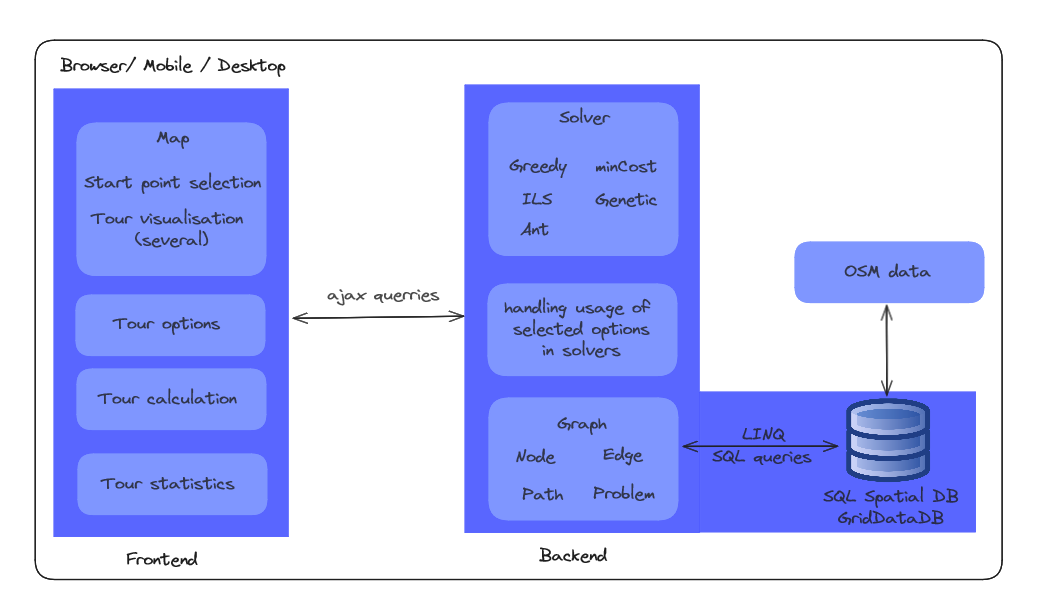
\includegraphics[width=1.1\textwidth]{bilder/Implementation Architecture.png}
	\caption{Visualization of the used architecture}
	\label{fig:architecture}
\end{figure}


In the above visualization, the whole application, the distinct parts and features as well as communications between them, are illustrated. 
The front-end runs as a web application in the browser but the visualization can also be customized to be executable as a mobile or desktop application (see section \ref{sec:futureWork}). 
In the visualized map, a marker can be set to the current location if the user grants permission to access their location data.
Searching for a specific address, drag-and-dropping the marker on the map, or scrolling the map and selecting a position by clicking on the place to mark are also possible. 
The visualization of the calculated tours is realized using the map and polygons built from the respective points.
These tours can be toggled on or off to allow for an easier overview after generating several tours.
For debugging purposes, there is a feature to show the entire graph that is being used for the calculation with the currently selected maximum length.

In addition to the map the front-end contains two menus:
One holding the parameters the user can use to customize the tours according to their preferences and the information menu containing a report of the core data of the calculated path that is being visualized. 
A more detailed description of the front-end design, concept sketches, and the final implementation are outlined in subsection \ref{subsec:interfaceAndFrontendChanges}.

The back-end manages all solvers that have been implemented, the database objects, and intermediate objects like the graph that is created from the nodes, edges, and their connections. 
The back-end also handles the parameters, selecting the correct solver, and generally managing the ajax requests received from the front-end. 
The database objects are generated when building the graph by accessing the database and using the stored values.

Finally, the database is filled using a python script that queries OSM-data to fetch all nodes and edges for a user-selected place.
For this example, data for Dortmund was retrieved.
Additionally, elevation data are obtained from a docker server using the latitude and longitude coordinates.



\subsection{Database}
\label{subsection:database}

The database is a relational database using Microsoft SQL server, administered in Microsoft SQL Server Management Studio.
This database supports spatial data, which is a crucial feature for storing and processing the nodes and edges.
Utilizing spatial features allows for filtering nodes within a specific radius, retrieving only a relevant subset of data points.
This filtering option within the database significantly enhances the data retrieval speed and the graph creation efficiency.
Compared to the previous method of generating a fixed graph for the city of Dortmund, the database offers further important advantages:
Far more nodes than only points within Dortmund can be used.
Although the database creation and the adding of points is relatively slow, this process is a one-time operation performed before the application is used and does not impact the tour calculation. 
Once the data has been added, all points can be accessed without needing to retrieve the entire database.

\paragraph{Gathering OSM data}

To create the database, a python script is used. 
This script first creates an osmnx graph from OSM data using the \texttt{graph\textunderscore from\textunderscore place} function
\begin{lstlisting}
	ox.graph\textunderscore from\textunderscore place(place\textunderscore name, network\textunderscore type='all', custom\textunderscore filter=custom\textunderscore filter)
\end{lstlisting}

In this script, the \texttt{place\textunderscore name} is the name of the city, state, country or region for which osmnx should gather the data points.
For a city, the city's name, state, and country need to be added. 
If a whole state should be selected, the state name and country are required.
The \texttt{network\textunderscore type} has six values to choose from\footnote{\url{https://osmnx.readthedocs.io/en/stable/user-reference.html\#module-osmnx.settings}, last accessed: 19.04.2024}: \texttt{all\textunderscore private}, \texttt{all}, \texttt{bike}, \texttt{drive}, \texttt{drive\textunderscore service}, and \texttt{walk}. 

The \texttt{custom\textunderscore filter} is defined to select only those edges, where walking, running, and cycling is possible by specifically de-selecting respective highway types:

\begin{lstlisting}
	custom_filter = '["highway"]["highway"!~"motorway|trunk|proposed|construction|motorway_link|trunk_link"]'
\end{lstlisting}

The excluded types are used for the following street types according to the OSM Wiki:
\begin{table}[ht]
	\centering
	\begin{tabular}{l|l}
		Highway type & Description\\
		\hline
		motorway & A restricted access major divided highway, normally with 2\\ 
		& or more running lanes plus emergency hard shoulder.\\
		& Equivalent to the Freeway, Autobahn, etc..  \\
		trunk & The most important roads in a country's system that aren't \\
		& motorways. (Need not necessarily be a divided highway.) \\
		proposed & For planned roads. \\
		construction & For roads under construction. \\
		motorway\textunderscore link & The link roads (sliproads/ramps) leading\\
		& to/from a motorway from/to a motorway or lower class highway. \\
		& Normally with the same motorway restrictions. \\
		trunk\textunderscore link & The link roads (sliproads/ramps) leading \\
		& to/from a trunk road from/to a trunk road or lower class highway. 
	\end{tabular}
	\caption[OSM highway types]{This table shows a listing of different OSM highway types and their definition taken from the Wiki page\protect\footnotemark}
	\label{tab:osmHighwayTypes}
\end{table}

\footnotetext{\url{https://wiki.openstreetmap.org/wiki/Key:highway}, last accessed: 19.04.2024}


\paragraph{Adding elevation data}

Next, the elevation data has to be added for the nodes of this graph.
These information are not part of osmnx and need to be retrieved from a different source.
For this thesis, Open Elevation\footnote{\url{https://open-elevation.com/}, last accessed: 20.03.2024} was used.
The data were downloaded and hosted in a local docker container that could be queried instead of the API.

Then, the surroundings information need to be obtained. 
These information are provided by OSM, however they are not saved for nodes.
A different query that retrieves areas and matches the respective tags to the saved nodes by matching the IDs has to be executed.

After gathering all the neccessary information, the script first checks if the database already contains matching tables and if not, generates them.
Then the nodes and edges that have been retrieved from osmnx can be iterated and inserted into the database using basic SQL.
During the iteration over the edges, the references between nodes and edges can be created (inserting edges into the IncidentEdges table that manages nodes and all their incident edges as well as adding references to the source- and target node when entering the edge data).
Using these references later enables the back-end code to easily access the endpoints of a graph or gather the incident edges for a node. 



\subsection{Interface and front-end changes}
\label{subsec:interfaceAndFrontendChanges}

The front-end was updated from the existing version of Tour4Me to allow for a better overview after adding several additional options for the user to select from. 
First, a conceptual idea (see figures \ref{fig:frontendConcept} to \ref{fig:frontendConceptResultsCloseup}) was built, mapping out the general structure of the new interface. 
The main changes focused on replacing the previous pop-ups through permanent menus.
On the side, a burger-menu button was added that allows for a side menu to be folded and unfolded to show the customization options (see figure \ref{fig:frontendSideMenuCloseups}). 
The result view was moved from an overlay on the map to a foldable footer menu (see figure \ref{fig:frontendConceptResultsCloseup}). 
Furthermore, the displayed tours and the respective information can now be unfolded additionally in this footer menu.
Previously, the tour information (including the length and other relevant data) was only accessible through a pop-up. 

Displaying all the resulting data while giving the option to fold and unfold them allows the user easier access and enables easier comparison between different tours.
Previously, only the data of a single tour could be shown in the pop-up. 
Now, the information of all tours are visible at the same time. 

\paragraph{Front-end concept}

\begin{figure}[H]
	\centering
	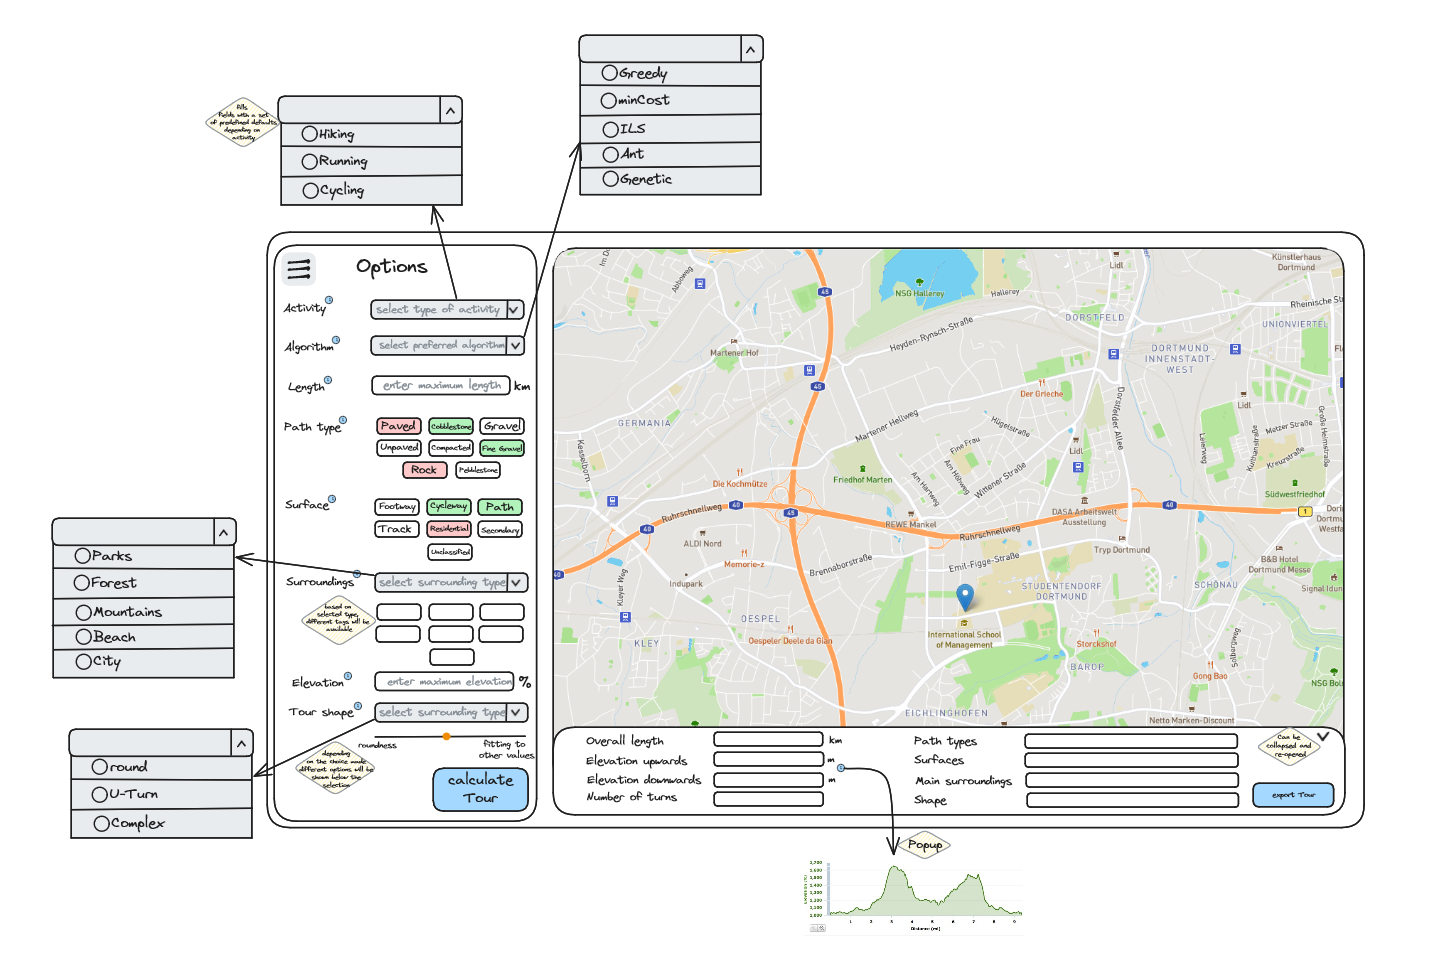
\includegraphics[width=0.9\linewidth]{bilder/Concept new Frontend design.png}
	\caption{Design concept for the front-end view, including descriptions for drop-downs and pop-ups}
	\label{fig:frontendConcept}
\end{figure}



The new interface has a more botanic color scheme, using mainly dark greens, browns, and blue while the text is off-white.
The side menu \textit{options} displays a wider selection of preference settings.
In figure \ref{fig:actualFrontendSideMenu}, the side menu is visualized. 
The uppermost drop down (see figure \ref{fig:actualFrontendSideMenuActivity}) can be used to set a pre-selection that fills in the following fields with suggested default values. 
These default values can always be customized afterwards but using default values can offer the user a higher usability.
The next selection shows all currently implemented algorithms (see figure \ref{fig:actualFrontendSideMenuAlgorithm}).
The resulting tours will turn out differently -- having higher importance on the covered area (roundness), or elevation and edge profit (see also chapter \ref{chapter:evaluation}) -- depending on the choice.
While greedy always prioritizes the maximum edge profit only and ignores the roundness of the tour, MinCost does the exact opposite.
Ant colony is more focused on edge profit, but also takes elevation and roundness into account.
Finally SA produces results that mostly focus on roundness while still taking edge profits and elevation into consideration. 
The respective combinations start with greedy, MinCost, or an empty solution and then strive to improve them. 

\paragraph{Implemented changes for the option menu}

All following options are direct tour parameters and describe user preferences.
The length is an estimate of the final tour length and is never used as a hard stop, but allows for tours to be within a range of a few hundred meters longer or shorter than the selected length.
However, tours are never more than a kilometer longer or shorter than the selected length.


The options for choosing the surface and the path type are implemented using selection buttons.
These buttons can be neutral (when they only show a white border), positive (colored in green) or negative (colored in red). 
A neutral button describes properties that are neither preferable nor undesirable while green marks preferred values and red marks undesired values.
Surfaces describe properties of the ground, path types characterize the type of street.
In OSM, there are many other options, however some are already filtered (for example highways) and others are not of significant interest and would only result in an overwhelmingly large selection.
To select desired or undesirable surroundings, a drop down menu has been implemented.
This menu allows the user to select a general type -- forest, grasslands, or other options -- that will then display the respective tags (see figure \ref{fig:actualFrontendSideMenuSurroundings}). 
This approach was used to minimize the number of tags and allow for an easier overview for the user.

The tour shape offers the options to choose a round tour, a U-turn, a complex tour, or do a custom selection (see \ref{fig:actualFrontendSideMenuTourShape}). 
Round tours have the highest importance (80 \%)on the roundness of a tour and split the remaining 20\% between elevation and edge profits. 
This makes rounder tours more likely to be calculated.
U-turns can have a special implementation that ensures for a slightly different path back to the beginning, but currently simply sets the importance of edge profits and elevation to 50\% each while ignoring the covered area completely through setting the respective importance to 0\%.
Complex tours are similar, but do not fully remove the importance of the area. 
For the custom selection, three sliders are displayed.
The slider inputs are linked so they influence each other, ensuring that the three probabilities always sum to 100\%.

Below the tour shape, elevation, and steepness can be selected. 
The elevation describes the maximum difference in elevation for the whole tour. 
This property does not differentiate between ascending or descending parts but sums up all differences and divides the overall result by two, to accommodate for the roundtrip. 
The steepness is used to exclude any part of the tour from being steeper than the chosen limit as much as possible.
With the inaccuracy of the elevation data, this can sometimes be impossible.
In these cases, creating any tour, even if it exceeds the limit is seen as more desirable than having no result at all.

At the bottom, the maximum runtime can be chosen, however no algorithm runs as long as 30 seconds with the current settings.
Clicking the button \enquote{Compute Path} will then send a query to the back-end, where all the selected information are processed, the matching solver is selected, and a tour is calculated.
The resulting roundtrip is then parsed into the latitude and longitude values of the nodes that form the tour and returned to the front-end.
Here, the latitude and longitude values can be displayed and connected to form a polygon that visualizes the resulting tour.

\begin{figure}[H]
	\centering
	\sbox{\measurebox}{%
		\begin{minipage}[b]{.25\textwidth}
			\subfloat
			[]
			{\label{fig:actualFrontendFullSideMenu}\includegraphics[height=0.5\textheight]{bilder/actualFrontendSideMenu.png}}
	\end{minipage}}
	\usebox{\measurebox}\qquad\hfill
	\begin{minipage}[b][\ht\measurebox][s]{.5\textwidth}
		\centering
		\subfloat
		[]
		{\label{fig:actualFrontendSurroundignsForest}\includegraphics[width=0.9\textwidth]{bilder/actualFrontendSideMenuSurroundingsForestSelected.png}}
		
		\vfill
		
		\subfloat
		[]
		{\label{fig:actualFrontendTourShapeCustomSliders}\includegraphics[width=0.9\textwidth]{bilder/actualFrontendSideMenuTourShapeCustomAndSlider.png}}
	\end{minipage}
	\caption{This figure shows the newly implemented side menu. (a) displays the full side menu (b) is a closeup of the surroundings when \textit{forest} is selected and (c) shows the three importance sliders when the selected tour shape is \textit{custom}}
	\label{fig:actualFrontendSideMenu}
\end{figure}

\paragraph{Route information overview}

All additional information are displayed in the \textit{Route information} footer menu. 
The menu as well as the calculated tours can be folded and unfolded.
This option does not decrease the size of the map but rather results in an added scroll-option, so the additional information can be displayed below the map.
The shown tours are colored in the same color as the respective displayed tour. 
A selection of ten colors is implemented, allowing for ten different tours to be calculated and displayed before a color is repeated. 
All of these colors are kept within the same botanical color scheme.
Next to the tour name, the used algorithm is written.
Furthermore, there is one button to toggle the visibility of the polyline in the leaflet map and one to delete the generated tour entirely.

\begin{figure}[H]
	\centering
	\includegraphics[width=0.9\textwidth]{bilder/routeInformationOneTour.png}
	\caption{This shows the Route information menu with one tour and all the related information unfolded and displayed}
	\label{fig:actualFrontendToureInfoMenuOneTour}
\end{figure}

Clicking on the tour name will fold (see figure \ref{fig:actualFrontendToureInfoMenuMoreTours}) and unfold (see figure \ref{fig:actualFrontendToureInfoMenuOneTour}) the respective information.
In this view, the final overall length, elevation, maximum steepness, collected Edge profits, total quality, covered area and for reference the maximum possible covered area independent of the calculated path.
On the right side, the collected path types and surfaces, surroundings, and the time it took to initialize the graph and to calculate the tour as well as the memory consumption are displayed.
The last three values are not of interest to the typical user but allow for a deeper insight into the calculation. 
Removing these outputs for a final version can be easily done if needed. 



\begin{figure}[H]
	\centering
	\includegraphics[width=0.5\textwidth]{bilder/routeInformationMoreTours.png}
	\caption{This shows the Route information menu with several folded tours displayed}
	\label{fig:actualFrontendToureInfoMenuMoreTours}
\end{figure}




\subsection{Parameter changes}
\label{subsec:parameterChanges}

To include the parameters that have been added in the front-end, a few minor changes had to be made to the existing algorithms. 
However, since MinCost already uses the quality calculation to determine the tours quality, nothing else had to be changed.
In the quality calculation the elevation difference, steepness difference, and the respective importance were added and the scaling was changed (see equation \ref{eq:qualitySA}).
Aside from that, more tags had to be added when creating the problem class, however this was done similarly to the existing tags (path type and surface) and did not need any further changes.
The greedy algorithm only takes the profit an edge can add into account and thus did not need any change.


\section{Algorithmic changes}
\label{sec:algorithmicChanges}

For the tour calculation, two new meta-heuristics were implemented.
The first one was ant colony, which was modified to match the AOP instead of TSP like the original.
The second meta-heuristic was a version of SA.
Here, the calculation of neighboring solutions had to be matched to return roundtrips.
In the following sections the changes that had to be made to result in implementations that can be applied to the AOP will be described.
For both meta-heuristics, the pseudocode and changed formulas will be explained.
The base idea and the overall working of the algorithms stays identical to the explanations in sections \ref{subsec:antColonyBackground} and \ref{subsec:simulatedAnnealingBackground}.


\subsection{Ant colony}
\label{subsec:antColonyImplementation}

For ant colony, several things had to be adjusted. 
First, for solving TSP, finding a shortest path and visiting all specified cities are the main objectives.
Whereas for AOP, these differ by a lot:
Here finding a \textit{matching} tour length that maximizes the profit is the important goal. 
Thus, the pheromone calculation, the trail intensity calculations, and the edge visibility had to be changed.

\paragraph{Pheromone calculation}

In the original paper, the pheromone amount to be placed on the collected edges was calculated based on the length of the tour the pheromone each ant can place on an edge. 
This scaling resulted in higher pheromone density for shorter tours and lower pheromone density for longer ones.
However, this constraint does not apply to the AOP.
Here, ideally all resulting tours should be approximately of the same length, close to the user-selected one.
Thus, the pheromone amount to be placed is based on the \texttt{edgeProfit} $p$ the edge with the length $l$ will grant the tour:


\begin{equation}
	\label{eq:newPheromoneCalc}
	\Delta\tau_{ij}^k = l(i,j) \cdot p(i,j) \cdot Q \text{ if (i,j)} \in \text{tour collected by the ant}
\end{equation}

The length of the edge from node \textit{i} to node \textit{j} is multiplied by the profits the same edge can collect based on the assigned tags, which is multiplied with the pheromone amount, a single ant can place on the trail ($Q$).
The latter is a means to scale the amount of pheromone placed and also enables the use of different ants for further combinations of ant colony, for example with genetic algorithms (see \ref{sec:futureWork}).
If the edge has a tag specified as desirable, the \texttt{edgeProfit} $p$ is increased by one.
If a tag that is specified as undesirabe, the profit will be decreased by one.
If the edge has no tag that is part of desirable or undesirable tags, the profit is 0.0001.
Like this, edges with desirabe tags will gain as much profit as they are long. 
Edges with undesirable tags will lower the profit by their length and edges without tags that are either desirable or undesirable, will impact the profit only by a fraction of their length.

\begin{equation}
	\label{eq:newProfitCalc}
	p(i,j) = \begin{cases}
		1 &\exists tag \in tags(i,j) \text{ tag} \in \text{desirable }\\
		-1 &\exists tag \in tags(i,j) \text{ tag} \in \text{undesirable }\\
		0.0001 &\text{ otherwise}
	\end{cases}
\end{equation}

\paragraph{Trail intensity calculation}

The trail intensity itself is calculated the same way as in the original paper (see \ref{eq:trailIntensity}).
However, for further calculations in the ant, it is scaled by dividing by the desired length $L$, based on whether or not an edge is visited twice:

\begin{equation}
	\label{eq:scaledTrailIntensity}
	\tau'_{i,j} = \begin{cases}
		 \frac{\tau_{i,j}}{L} &\text{edge already visited}\\
		\tau_{i,j} &\text{ otherwise}
	\end{cases}
\end{equation}

These updated values are not saved or used for other ants but saved in a separate set, so the penalty will only be applied for the ant that visits the edge twice.

\paragraph{Visibility calculation}

Furthermore, the visibility cannot be based on the length like the original paper did, since all tours should result in a length close to the desired one.
Thus, for the visibility, the edge quality is determined.
To calculate the quality, all selectable values have to be taken into account:
The \texttt{coveredArea} $A$, that maps the roundness of the tour, and the respective selected importance $i_A$, the \texttt{edgeProfit} $p$, and the respective selected importance $i_p$ as well as the elevation difference $e$ from the maximum $e_{max}$ summed with the steepness difference $s$ from the maximum $s_{max}$ and the respective importance $i_e$:

\begin{equation}
	\label{eq:newEdgeVisibility}
	\begin{split}
	\nu_{ij}^k = i_A \cdot 100 \cdot \frac{\sqrt{|A|\cdot \pi} \cdot 2 }{L} 
	+  i_p \cdot 100 \cdot p
	+ i_e \cdot \left(\frac{e_{max} - e}{e_{max}} + \frac{s_{max} - s}{s_{max}}\right)
	\end{split}
\end{equation}

The respective importance values are multiplied by 100 to scale them from the percentage values to be bigger than one. 
For the \texttt{covereArea}, the square root is taken in order to scale the size and account for the quadratic increase. 
The whole area is then scaled by the desired length of the tour $L$ to account for the larger value the area will have compared to the edge profits. 
The full derivation of the calculation of the scaling is shown in equations \ref{eq:scaleArea1} and \ref{eq:scaleArea2}, where A is the area and C is the circumference of a circle.


\begin{minipage}[t][2.5cm][b]{0.4\textwidth}
	\begin{equation}
		\label{eq:scaleArea1}
		\begin{split}
			C &= 2 \cdot \pi \cdot r\\
			\frac{C}{\pi \cdot 2} &= r\\
		\end{split}
	\end{equation}
\end{minipage}
\begin{minipage}[t][2.5cm][b]{0.4\textwidth}
	\begin{equation}
		\label{eq:scaleArea2}
		\begin{split}
			A &= \pi r^2 \\
			A &= \pi \cdot \left(\frac{C}{\pi \cdot 2}\right)^2\\
			A &= \pi \cdot \frac{C^2}{\pi^2 \cdot 2^2}\\
			A &= \frac{C^2}{\pi \cdot 4}\\
			A \cdot \pi \cdot 4 &= C^2\\
			\sqrt{A \cdot \pi} \cdot 2 &= C
		\end{split}
	\end{equation}
\end{minipage}

\paragraph{Probability calculation}

As in the original paper by Dorigo et al. \cite{dorigo_ant_1996}, the probabilities for the edges are calculated using the visibility and the trail intensity as well as the two parameters $\alpha$ and $\beta$ (see also \ref{eq:transitionProbability}), however, here, the scaled value $\tau'_{ij}$ is used:

\begin{equation}\label{eq:transitionProbability2}
	p_{ij}^k = \begin{cases}
		\frac{[\tau'_{ij}(t)]^{\alpha} \cdot [\nu_{ij}]^{\beta}}{\sum_{k \in allowed_k} [\tau'_{ij}(t)]^{\alpha} \cdot [\nu_{ij}]^{\beta}} &\text{if $j \in allowed_k$ }\\
		0 &\text{otherwise}
	\end{cases}
\end{equation}

\paragraph{Other changes}

Additionally, there is no tabuList and thus, this list cannot be used as a stopping criterion. 
Instead, a set number of tours are calculated.
Furthermore, the ants do not need to save the length of their current tour, as that value is not of any importance for the AOP version. 
Instead, the full quality of a tour is calculated and saved, so the best found tour for all ants can be determined.
The ants all have to start at the same position rather than in n different towns. 
The full updated pseudocode is shown in \ref{alg:AntColonyImplementation}


\begin{breakablealgorithm}
	%\begin{algorithm}[ht]
	\caption{AntColonyAOP}
	\label{alg:AntColonyImplementation}
	\begin{algorithmic}[1]
		\STATE initialize graph and problem (starting point, graph with nodes max $\frac{2}{3} \cdot L$ distance)
		\STATE init trailIntensity $\tau_{ij} \gets 0.0001$ for all edges(i,j)
		\STATE set starting pheromone values $pheromone(i,j) \gets 0$ for all edges(i,j)
		\STATE generate ants
		\STATE set current node $\gets$ starting point
		\FOR{\# runs}
		\FOR{\# ants}
		\STATE get all incident edges for current Node
		\WHILE{edge that doesn't exceed maximum length can be found}
		\FOR{edge (i,j) in incident edges}
		\STATE scale edge if already visited ($\tau'_{i,j}$)
		\STATE calculate \texttt{quality} which resembles the edge visibility using \ref{eq:newEdgeVisibility}
		\ENDFOR
		\STATE calculate probability to pick the edge based on \ref{eq:transitionProbability2} and scale them to sum to 1
		\STATE pick edge based on probability
		\STATE calculate new pheromone values for the picked edge according to \ref{eq:newPheromoneCalc}
		\STATE move current node to neighbor according to picked edge 
		\STATE add edge and node to solution lists
		\ENDWHILE
		\ENDFOR
		\STATE update trail intensities according to \ref{eq:trailIntensity}
		\STATE pick tour with best quality to use for next run
		\ENDFOR
		\STATE pick tour with best quality as result
	\end{algorithmic}	
	%\end{algorithm}
\end{breakablealgorithm}

To calculate the new ant colony implementation, the graph and a helper class \texttt{problem} have to be initialized first. 
The graph is created from the database, using the selected starting point and $\frac{2}{3} \cdot L$ to only fetch the needed number of nodes and edges.
The problem saves all other user inputs:


\begin{minipage}[t][2cm][b]{0.3\textwidth}
	\begin{itemize}
		\item desirable tags
		\item undesirable tags
		\item max tour length
	
	\end{itemize}
\end{minipage}
\begin{minipage}[t][2cm][b]{0.3\textwidth}
	\begin{itemize}
		\item quality (initially 0)
		\item max elevation
		\item max steepness
	\end{itemize}	
\end{minipage}
\begin{minipage}[t][2.9cm][b]{0.33\textwidth}
	\begin{itemize}
		\item elevationImportance
		\item edgeProfitImportance
		\item coveredAreaImportance
		\item generated solution path
	\end{itemize}	
\end{minipage}

\vspace{1cm}
The edges hold their length, the profit according to the tags, their pheromone and trail intensity. 
Here, the trail intensity is initialized with 0.0001 as a starting value, so all edges are equally as likely to be picked, however the value has to be bigger than 0 for the probability calculation.
As in the original paper, the pheromone are initialized with 0.

The ants can then be created and initialized. 
All ants use the same $\alpha$ and $\beta$ as well as the same base amount of pheromone they can distribute.
However, the values could be changed throughout the runs, which can be of interest for further combinations.

For a set number of runs, all ants calculate a tour in parallel. 
To do this, they all start at the selected starting point and then iteratively check the incident edges.
Only edges that can fully be traversed while not exceeding the maximum length selected will be used here.
If no edge is short enough to still fit into the tour, the roundtrip will be closed by calculating the shortest path from the last picked node back to the beginning.
While some edges are still available, they are scaled and then their visibility, and based on that the probability to choose the edge is calculated. 
Based on these probabilities, one edge is picked, the pheromone values are updated and the ant is moved.
The current node is updated accordingly. 
Finally, the picked edge and the new node can be added to the current solution.

After all ants have calculated their full tours, the overall trail intensity is updated, using the evaporation rate and the gathered pheromone updates from all ants. 
Then, the tour with the highest quality value is picked for further calculation. 
After the last run the tour with the highest probability is chosen as the final result.



\subsection{Simulated Annealing}
\label{subsec:simulatedAnnealingImplementation}

For SA, all needed changes are for the variables that are meant to be determined based on the problem which is to be solved with SA:
\begin{itemize}
	\item the quality of a solution
	\item how to find a neighboring solution
	\item the initial temperature and the cooling schedule
\end{itemize} 

Thus, the pseudocode does not change by much, however with that, the exact calculations can be specified. 
The updated pseudocode only additionally contains building the waypoint list, calculating distances and probabilities (see\ref{alg:SAImplementation})

\paragraph{Quality calculation}

The quality $f(j)$ of the solution $j$ is -- like for ant colony -- calculated based on the \texttt{coveredArea} $A$ and the respective importance (\texttt{coveredAreaImportance} $i_A$), the \texttt{edgeProfit} $p$ and the respective importance (\texttt{edgeProfitImportance} $i_p$), and the elevation difference $e$ from the maximum $e_{max}$ and the respective importance $i_e$ and scaled by the difference between the actual length $L_{calc}$of the tour from the target length (L). 

\begin{equation}
	\label{eq:qualitySA}
	\begin{split}
		f(j) = \frac{i_A \cdot 100 \cdot \frac{\sqrt{|A|\cdot \pi} \cdot 2 }{L} 
		+  i_p \cdot 100 \cdot p
		+ i_e \cdot \left(\frac{e_{max} - e}{e_{max}} + \frac{s_{max} - s}{s_{max}}\right)}{\left| L - L_{calc} \right|}
	\end{split}
\end{equation}

The respective importance values are again multiplied by 100 and the  \texttt{coveredArea} is scaled the same as for the ant colony (see \ref{eq:visibility}, \ref{eq:scaleArea1} and \ref{eq:scaleArea2})

\paragraph{Determining a neighboring solution}

The neighboring solution is created based on waypoints, which are used similarly to how they work in the MinCost tour creation (see \ref{subsec:Tour4Me}):
A the waypoints form base points of the tour are connected using a weighted version of shortest paths. 
For this calculation, the shortest path of any point to the starting point is determined by dividing the edge length by the profit that can be gained when choosing the edge. 

For SA, several different versions have been implemented.
The first two that are described here start with an empty tour and build the solution with only the starting point.
In the next section, other combinations and alterations are discussed as well.

The two versions that start with an empty solution are a weighted and a fully random version of the same base idea:
A random point (with or without a probability distribution) is picked as a new waypoint. 
Until at least five waypoints have been found, adding or moving a waypoint are the only options available, however when only one waypoint exists, a second one \textit{must} be added first.
After that, adding, moving, and removing of a waypoint are possible until 15 points are reached.
After that, a waypoint can only be moved or removed.
Using these boundaries ensures that the resulting tour will not end up too short while also assuring that not too many distance calculations are needed.
The number of waypoints determines how many times the distance of a new waypoint is of interest, since for moving, and adding, the closest existing waypoint has to be known.

\paragraph{Using waypoints}

Whether a waypoint is moved, removed, or a new one is added is picked randomly within the previously given constraints.
The starting point can neither be chosen for moving nor for removing.

First, a random point is selected from the set of available nodes.
This set is a smaller version of all available nodes, allowing only nodes that have a shortest distance of at most $\frac{L}{4}$ from the starting point. 
For the version using a probability distribution, the probabilities are calculated using a scaled version of the distance of every point $j$ from the starting point $s$: $dist(j,s)^2$.
For the fully random version, a distance of 1 is used for every edge.
Every point that is too far from the starting point is assigned 0 and will be removed from the returned result.
The respective calculated distances are then scaled by the sum of all distances to sum to 1.

The final selected point is the new waypoint candidate for moving or adding and will determine the waypoint to choose, also for the remove case (see figures \ref{fig:tour_picked_waypoint_shortest_paths}-\ref{fig:shortestPathAndRemoveDone} for a visualization of all options and how these operations alter the tour).
To pick the waypoint that will be moved or removed or to find the two waypoints between which the new point should be added, all distances have to be calculated.
The closest waypoint of the current list will then be picked as visualized in the following figures:
%
%	\begin{figure}[H]
%		\centering
%		\includesvg[width=0.7\linewidth]{bilder/add_move_remove/tour&waypoint.svg}
%		\caption{This figure shows the path, which is separated in ten waypoints (red) and a new random point (green)}
%		\label{fig:waypoint}
%	\end{figure}
	\begin{figure}[H]
		\centering
		\includesvg[width=0.7\linewidth]{bilder/add_move_remove/tour_picked_waypoint_shortest_paths.svg}
		\caption{This figure shows the path, which is separated in ten waypoints, a new random point and four of the distances to the closest waypoints.}
		\label{fig:tour_picked_waypoint_shortest_paths}
	\end{figure}

The two illustrations show a path (black outline) with ten waypoints that are evenly distributed.
In the figure, a random point that has been picked for the following steps is highlighted in green.
Additionally, four distances to the nearest waypoints from the path are highlighted using the four green lines from the new point to the respective four closest waypoints.
The third connection from the top is the shortest one, indicating the closest waypoint.

After picking a waypoint, three options are available.
These moves are listed and explained in the following.
Illustrations for each move are given below.


\begin{itemize}
	\item \textbf{added:} from the two neighbors of the selected waypoint, the closest one is picked and the new point is added in between, updating the path between the overall closest point to be the shortest path between the waypoint and the new point and updating the path between the closer one of the neighboring waypoints to be the shortest path between the new point and that waypoint (see \ref{alg:SAGenerateNeigborhoodAdd})
	\item \textbf{moved:} the previous waypoint is deleted, a new shortest path from the predecessor to the new point and a shortest path from the new point to the successor is calculated and the new point is added as the moved version of the selected waypoint (see \ref{alg:SAGenerateNeigborhoodMove})
	\item \textbf{removed:} the picked waypoint is deleted and a new shortest path between the predecessor and the successor is calculated (see \ref{alg:SAGenerateNeigborhoodRemove})
\end{itemize}


\paragraph{Adding a waypoint}
This move is visualized in the following to figures.
The first illustration (\ref{fig:shortestPathAndAdd}) highlights the distances to the closest waypoint and the closer one of the respective neighbors.
As shown in figure \ref{fig:tour_picked_waypoint_shortest_paths}, the second connection from the top would be shorter than the fourth one, which was chosen in this figure.
This choice stems from the fact that only the single closest waypoint is of interest for the initial selection. 
For every following move, only the respective neighbors can be used for any operation afterwards.
The process of adding a waypoint changes the path between the closest waypoint on the existing line and the closer one of the respective neighbors. 
This path fragment is removed, which is indicated by crossing out the part of the previous path in figure \ref{fig:shortestPathAndAdd}.
In illustration \ref{fig:shortestPathAndAddDone}, the new, changed path is visualized.
All previous waypoints are still on the path, but the changed fragment (highlighted in blue) now includes the additional waypoint.

	\begin{figure}[H]
		\centering
		\includesvg[width=0.7\linewidth]{bilder/add_move_remove/waypoint,shortest_path&neighbors-add.svg}
		\caption{This figure shows the path, the randomly picked point and the path to the closest waypoint.
			The random point will be added between the closest waypoint and the respective closest neighbor.
			The path fragment that will be changed through adding is crossed out.}
		\label{fig:shortestPathAndAdd}
	\end{figure}
	\begin{figure}[H]
		\centering
		\includesvg[width=0.7\linewidth]{bilder/add_move_remove/waypoint,shortest_path&neighbors-changed_after_add.svg}
		\caption{This figure shows the path after the waypoint was added.}
		\label{fig:shortestPathAndAddDone}
	\end{figure}
	

\paragraph{Moving a waypoint}	
The process of moving a waypoint includes in principle removing one existing waypoint and adding in the new random point. 
Figure \ref{fig:shortestPahtAndMove} visualizes the closest waypoint on the current path.
The dashed arrow indicates how this chosen waypoint will be moved towards the new point.
For this move, both adjacent path fragments have to be updated.
The new path with the moved waypoint is illustrated in figure \ref{fig:shortestPathAndMoveDone}.
The previous waypoint is still visualized, but not part of the path anymore.
The new waypoint is included on the path and both adjacent path fragments are updated.
	
	
	\begin{figure}[H]
		\centering
		\includesvg[width=0.7\linewidth]{bilder/add_move_remove/waypoint,shortest_path&neighbors-move.svg}
		\caption{This figure shows the path, the randomly picked point and the path to the closest waypoint, which will be moved following the arrow to the random point.
			The path fragment that will be changed through moving is crossed out.}
		\label{fig:shortestPahtAndMove}
	\end{figure}
	\begin{figure}[H]
		\centering
		\includesvg[width=0.7\linewidth]{bilder/add_move_remove/waypoint,shortest_path&neighbors-changed_after_move.svg}
		\caption{This figure shows the path after the waypoint was moved.}
		\label{fig:shortestPathAndMoveDone}
	\end{figure}
	

\paragraph{Removing a waypoint}
To remove a waypoint, technically no new point is needed. 
However, choosing a random point and determining the closest waypoint is using the same mechanism as for adding and moving, which keeps the used methods consistent.
While it would be possible to pick and remove one of the waypoints without finding and using a random point, this approach would be an entirely different concept, ignoring the probability distributions used to determine a new random point.
Thus, illustration \ref{fig:shortestPahtAndRemove} is very similar to figure \ref{fig:shortestPahtAndMove}.
Only the arrowhead is missing since the closest waypoint is not moved but removed from the path.
For this move, again both neighboring path fragments have to be updated.
The resulting path -- containing neither the random point nor the previous waypoint -- is visulaized in illustration \ref{fig:shortestPathAndRemoveDone}.


	\begin{figure}[H]
		\centering
		\includesvg[width=0.7\linewidth]{bilder/add_move_remove/waypoint,shortest_path&neighbors-remove.svg}
		\caption{This figure shows the path, the randomly picked point and the path to the closest waypoint.
		The path fragment that will be changed through removing is crossed out.}
		\label{fig:shortestPahtAndRemove}
	\end{figure}
	\begin{figure}[H]
		\centering
		\includesvg[width=0.7\linewidth]{bilder/add_move_remove/waypoint,shortest_path&neighbors-changed_after_remove.svg}
		\caption{This figure shows the path after the waypoint was removed.}
		\label{fig:shortestPathAndRemoveDone}
	\end{figure}





For the new tour, the overall quality is calculated using \ref{eq:qualitySA}. 
Then, if the quality is better than the one of the previous tour, the new tour will always be accepted.
If the quality is worse, the probability with which the tour is accepted anyways is calculated based on \ref{eq:SAprobCalculation}. 
This step is done for a set number of inner runs, before the temperature is adjusted based on \ref{eq:temperatureSchedule}.




To better illustrate the added steps to choosing and building a solution, the pseudocode fo the inner loop is given in \ref{alg:SAGenerateNeigborhood}:



\begin{breakablealgorithm}
	\caption{Generate neighborhood roundtrip j}
	\label{alg:SAGenerateNeigborhood}
	\begin{algorithmic}[1]
		\STATE pick random waypoint based on probability distribution
		\STATE calculate all distances to current waypoints and pick closest
		\IF{\# waypoints < 3}
		\STATE add new waypoint between closest and that waypoint's closest neighbor
		\ELSE \IF{\# waypoints $\leq$ 5}
		\STATE randomly decide if to add or move
		\ELSE \IF{5 < \# waypoints < 15 }
		\STATE randomly decide if to add, remove or move
		\ELSE 
		\STATE randomly decide if to remove or move
		\ENDIF
		\ENDIF
		\ENDIF
		\STATE calculate new quality
		\STATE return new solution
	\end{algorithmic}
\end{breakablealgorithm}


\subsection{Combinations}
\label{subsec:algoCombinations}

In addition to the pure versions of Ant Colony and SA, a few combinations with the two existing algorithms (Greedy and MinCost) as well as a combination of first using ant colony and then applying SA have been implemented.
For this, only small changes had to be made to the existing code base, which will be shortly illustrated in the following paragraphs.

\paragraph{Ant + Greedy and Ant + MinCost}

To realize the combination of ant with the two already implemented algorithms, the changes are minor.
First, the respective algorithm has to be run to create a base tour to build the ant algorithm from.
Then, the initialization has to place trail intensity and pheromone on the edges of the existing tour.
Lastly, the importance of the trail intensity has to be higher than in the pure ant algorithm to make it more likely that the ants will follow the previous tour.


\paragraph{SA + Greedy, SA + MinCost, SA + Ant}

To implement the combinations with SA, the tours have to be calculated first.
Then, the waypoint list can be created from the base tour that has been built, splitting the tour into 10 waypoints and the paths connecting them. 
Other than that, no changes are needed.

%Realizing combinations is relatively easy for the given variations, however more complicated combinations are possible.
%Especially combining a genetic meta-heuristic could result in more complex ways of combining algorithms and result in interesting new solutions. 
%This could not be implemented due to time constraints, however possible approaches are discussed in the section about future work (\ref{sec:futureWork}).
